\RequirePackage{amsmath}
\documentclass[twocolumn, times]{aastex631}
\usepackage[spanish,es-minimal,english]{babel}
\usepackage[utf8]{inputenc}
\usepackage{natbib}
%\usepackage{microtype}
\usepackage{hyperref}
\usepackage{savesym}
\savesymbol{tablenum}
\usepackage{siunitx}
\restoresymbol{SIX}{tablenum}
\usepackage[varg]{newtxmath}
\usepackage{newtxtext}
\usepackage{booktabs}
\usepackage{array}   % for \newcolumntype macro
\newcolumntype{L}{>{$}l<{$}} % math-mode version of lrc column types
\newcolumntype{R}{>{$}r<{$}} 
\newcolumntype{C}{>{$}c<{$}} 

\bibliographystyle{aasjournal}

\newcommand\ION[2]{#1\,\scalebox{0.9}[0.8]{\uppercase{#2}}}
\newcounter{ionstage}
\renewcommand{\ion}[2]{\setcounter{ionstage}{#2}% 
  \ensuremath{\mathrm{#1\,\scriptstyle\Roman{ionstage}}}}
\newcommand\hii{\ion{H}{2}}
\newcommand\heii{\ion{He}{2}}
\newcommand\hei{\ion{He}{1}}
\newcommand\sii{[\ion{S}{2}]}
\newcommand\oiii{[\ion{O}{3}]}
\newcommand\ariv{[\ion{Ar}{4}]}
\newcommand\Raman{\ensuremath{_{\text{Raman}}}}
\def\th#1#2{\(\theta^{#1}\)\,Ori~#2}
\newcommand\wn{\ensuremath{\tilde{\nu}}}

% Chemical formulae
\newcommand*\chem[1]{\ensuremath{\mathrm{#1}}}
% Atomic term symbols
\newcommand\Config[1]{\ensuremath{\mathrm{#1}}}
\newcommand\Term[3]{\ensuremath{\mathrm{#1\ ^{#2}#3}}}
\newcommand\Level[4]{\ensuremath{\mathrm{#1\ ^{#2}#3_{#4}}}}

\newcommand\ha{\ensuremath{\text{H}\alpha}}
\newcommand\lya{\ensuremath{\text{Ly}\alpha}}
\newcommand\lyb{\ensuremath{\text{Ly}\beta}}

\begin{document}
\title{A highly ionized stellar bow shock in the Small Magellanic Cloud}
\shorttitle{Highly ionized bow shock in LMC}
\author{William J. Henney and S. Jane Arthur}
\affiliation{%
  \foreignlanguage{spanish}{Instituto de Radioastronomía y
    Astrofísica, Universidad Nacional Autónoma de México, Apartado
    Postal 3-72, 58090 Morelia, Michaoacán, Mexico}}
\email{w.henney@irya.unam.mx}

\begin{abstract}
  We report the discovery of a parsec-scale stellar bow shock
  associated with the O2\,III(f) star Walborn~3
  in the cluster NGC~346 of the Small Magellanic Cloud.
  Emission line images of \ion{He}{2} and [\ion{Ar}{4}], etc.
\end{abstract}

\keywords{Atomic physics; Radiative transfer; Photodissociation regions}

%\object{M42}

\section{Introduction}
\label{sec:introduction}




\section{Observations}
\label{sec:observations}


\begin{figure*}
  \centering
  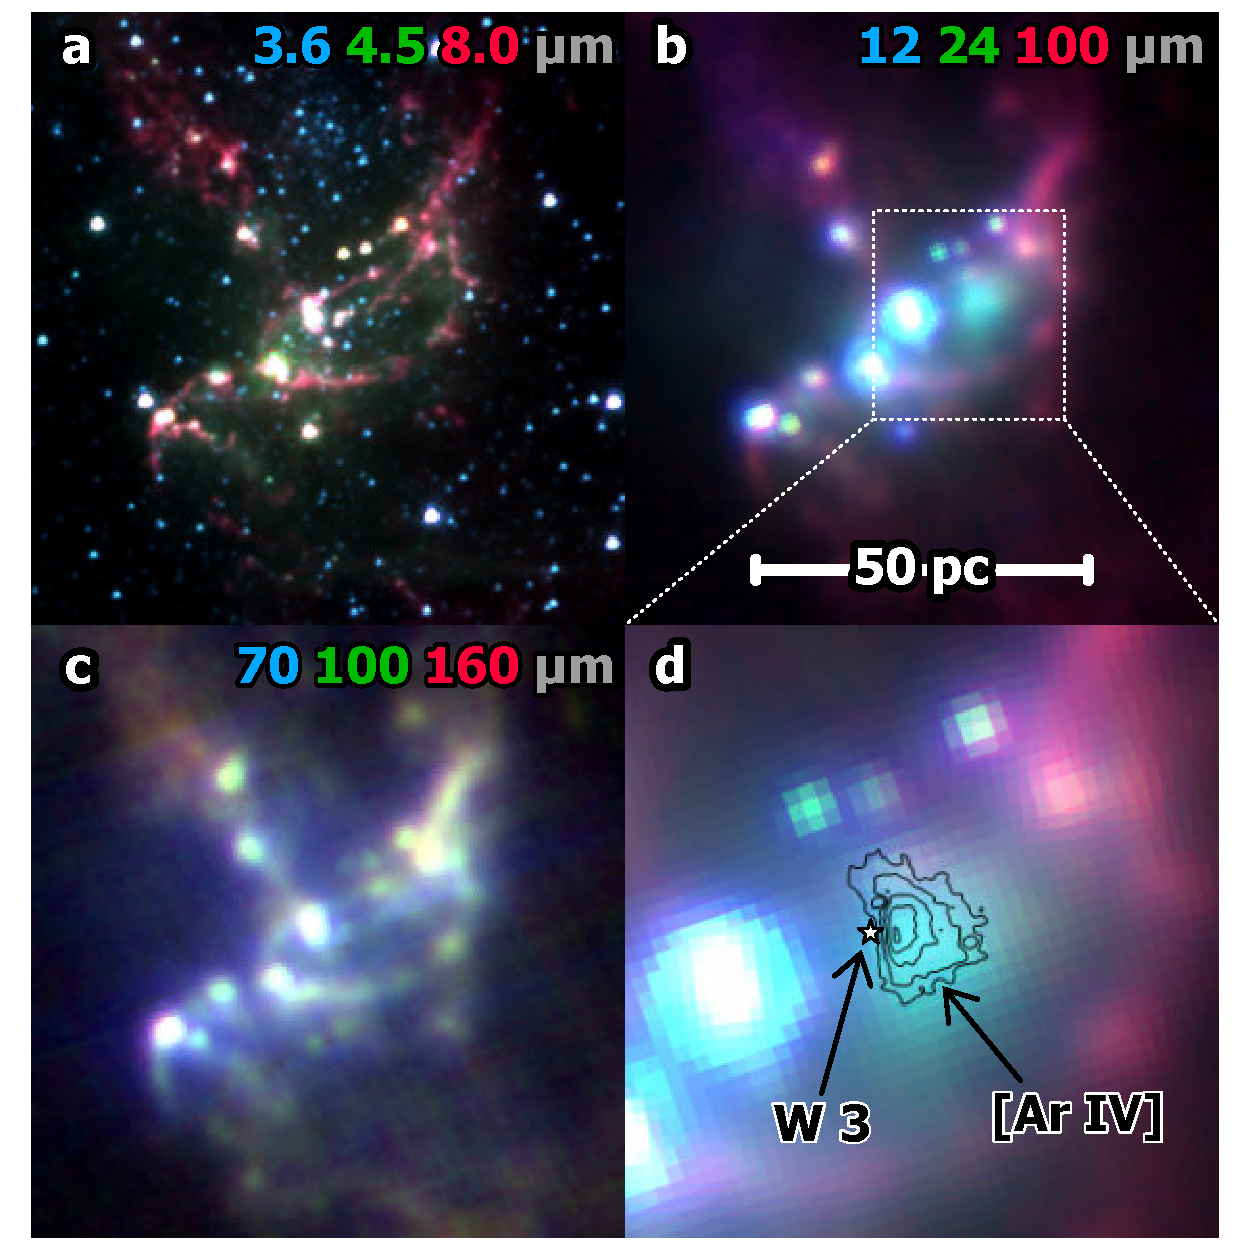
\includegraphics[width=\linewidth]{figs/ngc346-infrared-multipanel}
  \caption{
    Infrared images of NGC 346.
    }
  \label{fig:infrared-multipanel}
\end{figure*}

\begin{figure}
  \centering
  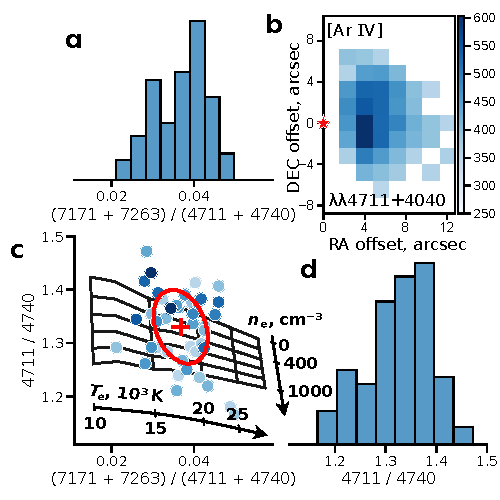
\includegraphics[width=\linewidth]{figs/ngc346-bow-shock-ariv-diagnostics-annotated}
  \caption{
    Temperature and density diagnostics of the bow shock from \ariv{} line ratios.
    }
  \label{fig:ariv-diagnostics}
\end{figure}

\section{Results}
\label{sec:results}


\section{Conclusions}
\label{sec:conclusions}

\begin{acknowledgments}
  Thank you.
\end{acknowledgments}

\facilities{VLT:Yepun (MUSE)}

\bibliography{smc-bow-refs}

\end{document}

%%% Local Variables:
%%% mode: latex
%%% TeX-master: t
%%% End:
